\subsection{The Goto Approach to Implementing {\sc gemm}}
\label{sec:BLIS}

\begin{figure}[tb!]
	\begin{center}
		\begin{minipage}{3in}
			\mbox{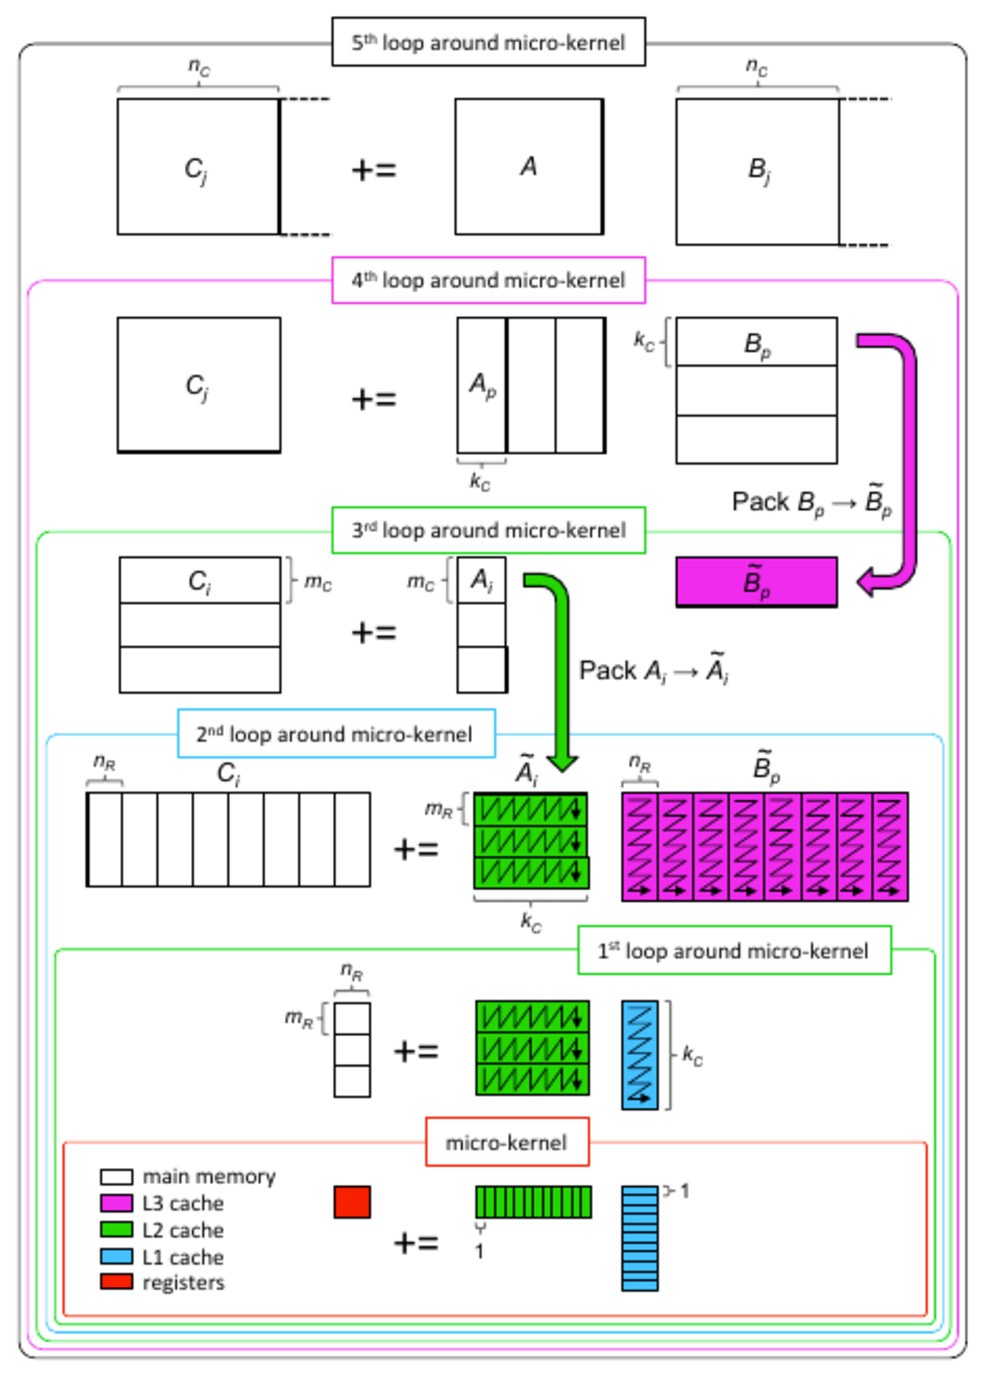
\includegraphics[width=3.0in]{mm_blis_color.pdf}}
		\end{minipage}
		~~~
		\begin{minipage}[t]{3in}
			\footnotesize  
			\mbox{\input blis_gemm_new  }
		\end{minipage}
	\end{center}
	\caption{Left: The Goto algorithm for matrix-matrix multiplication as  
		refactored in BLIS.  Right: the same algorithm, but expressed as  
		loops.}
	\label{fig:blis_gemm}
\end{figure}

Around 2000, Kazushige Goto revolutionized how \Gemm\ is implemented on current CPUs with his techniques
that were first published in the paper
\begin{quote}
	Kazushige Goto, Robert A. van de Geijn.\\
	\href{http://dl.acm.org/citation.cfm?id=1356052.1356053&coll=DL&dl=GUIDE&CFID=71223967&CFTOKEN=96440140}{Anatomy of high-performance matrix multiplication.}\\
	ACM Transactions on Mathematical Software (TOMS).\\
	Volume 34 Issue 3, May 2008, Article No. 12.
\end{quote}
A further "refactoring" of this approach was more recently described in 
\begin{quote}
	Field G. Van Zee, Robert A. van de Geijn. \\
	\href{http://dl.acm.org/citation.cfm?id=2786970.2764454&coll=DL&dl=GUIDE&CFID=702354034&CFTOKEN=48470379}{%
		BLIS: A Framework for Rapidly Instantiating BLAS Functionality.} \\
	ACM Transactions on Mathematical Software (TOMS).\\
	Volume 41 Issue 3, June 2015,
	Article No. 14.
\end{quote}
The advantage of the BLIS framework is that it reduces the kernel that must be highly optimized, possibly with vector intrinsics or in assemply code, to a {\em micro-kernel}. 

The 


\subsection{Set up}

\begin{figure}[tb!]
	\begin{center}
\begin{minipage}{4in}
	\dirtree{%
		.1 step3.
		.2 README 
%%%\DTcomment{
%%%  \rm \color{red}
%%%  contents of the directory, how to compile and execute the source code{.} 
%%%}
.
		.2 sourceme.sh 
%%%\DTcomment{
%%%			\rm \color{red}
%%%			comment{.} 
%%%		}
.
		.2 makefile 
%%% \DTcomment{
%%%			\rm \color{red}
%%%			comment{.} 
%%%		}
.
		.2 dgemm 
%%%\DTcomment{
%%%			\rm \color{red}
%%%			comment{.} 
%%%		}
.
		.3 my\_dgemm.c 
%%% \DTcomment{
%%%			\rm \color{red}
%%%			comment{.} 
%%%		}
.
		.3 bl\_dgemm\_ref.c 
%%%\DTcomment{
%%%			\rm \color{red}
%%%			comment{.} 
%%%		}
.
		.3 bl\_dgemm\_util.c 
%%% \DTcomment{
%%%			\rm \color{red}
%%%			comment{.} 
%%%		}
.
		.2 include 
%%%\DTcomment{
%%%			\rm \color{red}
%%%			comment{.} 
%%%		}
.
		.3 avx\_types.h 
%%% \DTcomment{
%%%			\rm \color{red}
%%%			comment{.} 
%%%		}
.
		.3 bl\_dgemm.h 
%%% \DTcomment{
%%%			\rm \color{red}
%%%			comment{.} 
%%%		}
.
		.3 bl\_dgemm\_ref.h 
%%%\DTcomment{
%%%			\rm \color{red}
%%%			comment{.} 
%%%		}
.
		.3 bl\_config.h 
%%% \DTcomment{
%%%			\rm \color{red}
%%%			comment{.} 
%%%		}
.
		.3 bl\_dgemm\_kernel.h 
%%% \DTcomment{
%%%			\rm \color{red}
%%%			comment{.} 
%%%		}
.
		.2 kernels
%%%\DTcomment{
%%%			\rm \color{red}
%%%			comment{.} 
%%%		}
.
		.3 bli\_dgemm\_ukr.c
%%%\DTcomment{
%%%			\rm \color{red}
%%%			comment{.} 
%%%		}
.
		.3 bli\_dgemm\_int\_d8x4.c
%%%\DTcomment{
%%%			\rm \color{red}
%%%			comment{.} 
%%%		}
.
		.3 bli\_dgemm\_asm\_d8x4.c
%%%\DTcomment{
%%%			\rm \color{red}
%%%			comment{.} 
%%%		}
.
		.3 bli\_dgemm\_asm\_d8x6.c
%%%\DTcomment{
%%%			\rm \color{red}
%%%			comment{.} 
%%%		}
.
		.3 bli\_dgemm\_asm\_d12x4.c
%%%\DTcomment{
%%%			\rm \color{red}
%%%			comment{.} 
%%%		}
.
		.2 lib 
%%%\DTcomment{
%%%			\rm \color{red}
%%%			comment{.} 
%%%		}
.
        .3 libblislab.a
%%% \DTcomment{
%%%			\rm \color{red}
%%%			comment{.} 
%%%		}
.
        .3 libblislab.so
%%% \DTcomment{
%%%			\rm \color{red}
%%%			comment{.} 
%%%		}
.
		.2 make.inc.files
%%% \DTcomment{
%%%			\rm \color{red}
%%%			comment{.} 
%%%		}
.
		.3 make.intel.inc 
%%% \DTcomment{
%%%			\rm \color{red}
%%%			comment{.} 
%%%		}
.
		.3 make.gnu.inc 
%%%\DTcomment{
%%%			\rm \color{red}
%%%			comment{.} 
%%%		}
.
		.3 make.inc 
%%% \DTcomment{
%%%			\rm \color{red}
%%%			comment{.} 
%%%		}
.
		.2 test 
%%%\DTcomment{
%%%			\rm \color{red}
%%%			comment{.} 
%%%		}
.
		.3 makefile 
%%% \DTcomment{
%%%			\rm \color{red}
%%%			comment{.} 
%%%		}
.
		.3 test\_bl\_dgemm.c 
%%%\DTcomment{
%%%			\rm \color{red}
%%%			comment{.} 
%%%		}
.
		.3 run\_bl\_dgemm.sh 
%%% \DTcomment{
%%%			\rm \color{red}
%%%			comment{.} 
%%%		}
.
		.3 test\_bl\_dgemm.x 
%%%\DTcomment{
%%%			\rm \color{red}
%%%			comment{.} 
%%%		}
.       
		.3 tacc\_run\_bl\_dgemm.sh 
%%% \DTcomment{
%%%			\rm \color{red}
%%%			comment{.} 
%%%		}
.	
	}
\end{minipage}
\end{center}
\caption{Structure of directory {\tt step3}.}
\label{fig:DirStep1}
\end{figure}

Figure~\ref{fig:DirStep1} illustrates the directory
structure for subdirectory {\tt step3}. Comparing to {\tt step2}, we have modified/added the following directories/files:

\begin{description}
\item[{\tt kernels}] This directory contains the micro-kernel implementations for various architecture.
\begin{description}
\item[{\tt bli\_dgemm\_int\_d8x4.c}] Is a {\tt AVX} intrinsics micro-kernel implementation for Sandy Bridge/Ivy Bridge micro-architecture.
\item[{\tt bli\_dgemm\_asm\_d8x4.c}] Is a {\tt AVX} assembly micro-kernel implementation for Sandy Bridge/Ivy Bridge micro-architecture.
\item[{\tt bli\_dgemm\_asm\_d8x6.c}] Is a {\tt AVX2} assembly micro-kernel implementation for Haswell micro-architecture.
\item[{\tt bli\_dgemm\_asm\_d12x4.c}] Is an alternative {\tt AVX2} assembly micro-kernel implementation for Haswell micro-architecture.
\end{description}
\end{description}


